\makeheading{Lecture 16 | 2020-11-04}
\section{Addressing Problems With Regression Model Assumptions}

If residual plots reveal problems with assumptions
(although plots don't fully check linearity, independence),
we might be able to address via \underline{transformations},
adding variables to model, using different error
distribution on $ \varepsilon $.
\begin{enumerate}[label=(\arabic*)]
      \item Variance-stabilizing transformations on
            responses $ y_i $, can help constant variance identified
            on $ \symbf{e} $ vs $ \hat{\symbf{\mu}} $ plot.

            \underline{Idea}: apply function $ g(\cdot) $ and fit
            regression on transformed $ g(y_i) $; that is,
            \[ g(Y_i)=\beta_0+\beta_1x_{i1}+\cdots+\beta_p x_{ip}+\varepsilon_i \]
            Note this can drastically change $ \SS{Res} $
            and $ \hat{\sigma} $, so cannot directly use those among different
            choices $ g(\cdot) $.

            \underline{Rationale}: variance of response might be a function
            of mean $ \mu_i=\E{Y_i} $; could be expressed
            \[ \Var{Y_i}=\Var{\varepsilon_i}=h(\mu_i)\sigma^2 \]
            for some $ h(\cdot)>0 $. In which case, we want
            \[ \Var{g(Y_i)}\approx \sigma^2 \]
            1st order Taylor expansion
            \[ g(Y_i)\approx g(\mu_i)+(Y_i-\mu_i)g^\prime(\mu_i) \]
            \[ \Var{g(Y_i)}\approx [g^\prime(\mu_i)]^2\Var{Y_i} \]
            Thus, for $ \Var{g(Y_i)} $ to be constant, we need
            \[ [g^\prime(\mu_i)]^2\propto \frac{1}{h(\mu_i)} \]
            Examples:
            \begin{enumerate}[label=(\roman*)]
                  \item $ h(\mu_i)=\mu_i $; that is,
                        $ \Var{Y_i}=\sigma^2 \mu_i\propto \mu_i $.
                        Variance in responses proportional to mean response.
                        We need
                        \[ g^\prime(\mu_i)\propto \frac{1}{\sqrt{h(\mu_i)}}=
                              \frac{1}{\sqrt{\mu_i}} \]
                        and so $ g(\mu_i)=\sqrt{\mu_i} $ works,
                        and we apply $ g(y_i)=\sqrt{y_i} $
                        to obtain approximately constant variance
                  \item $ h(\mu_i)=\mu_i^2 $; that is,
                        $ \Var{Y_i}=\sigma^2\mu_i^2 \propto \mu_i^2 $
                        or
                        $ \Sd{Y_i}\propto \mu_i $.
                        We need
                        \[ g^\prime(\mu_i)\propto\frac{1}{\mu_i} \]
                        and so $ g(\mu_i)=\ln(\mu_i) $ works, and we apply
                        $ g(y_i)=\ln(y_i) $
                        to stabilize variance.
                  \item Class of power transformations (Box-Cox)
                        \[ g(y_i)=\begin{dcases}
                                    \frac{y_i^\lambda -1}{\lambda} & \lambda\neq 0 \\
                                    \ln(y_i)                       & \lambda=0
                              \end{dcases} \]
                        \[ g^\prime(\mu_i)=\begin{dcases}
                                    \mu_i^{\lambda-1} & \lambda\neq 0 \\
                                    \frac{1}{\mu_i}   & \lambda=0
                              \end{dcases}\iff h(\mu_i)\propto \frac{1}{[g^\prime(\mu_i)]^2}
                              =\mu_i^C \quad {C\in\mathbf{R}}  \]
                        Box-Cox transformation can help address non-constant
                        variance of the form
                        \[ \mu_i^C\sigma^2=\Var{Y_i} \]
                        Special cases include:
                        \begin{itemize}
                              \item $ \displaystyle \lambda=\frac{1}{2} $ is $ \sqrt{\cdot} $
                              \item $ \lambda=0 $ is $ \ln(\cdot) $
                              \item $ \lambda=1 $ is identity
                              \item $ \lambda=-1 $ is reciprocal
                        \end{itemize}
                        can automatically try a sequence of $ \lambda $
                        and find the choice that gives the best value of
                        likelihood
            \end{enumerate}
            Note that interpreting $ \hat{\beta}_j $ can be less intuitive
            as a result of transformation, since now increasing $ x_j $
            by $ 1 $ unit corresponds to an estimated change of $ \hat{\beta}_j $
            in $ g(y_i) $. For $ g(y_i)=\ln(y_i) $, $ \hat{\beta}_j $
            represents estimate of expected change in $ \ln(y_i) $
            which corresponds to $ e^{\hat{\beta}_j} $ being
            the expected multiplicative change applied to the (original)
            response. But for an arbitrary $ \lambda $, the transformation
            might be less interpretable.
      \item Transforming and/or adding explanatory variables.
            \begin{itemize}
                  \item If $ y $ (or $ g(y) $) has a clear non-linear
                        relationship with some $ x_j $, we can consider transforming
                        $ \symbf{x}_j $ (e.g. $ \ln(\cdot) $, $ \sqrt{\cdot} $, etc.)
                  \item Could add polynomial terms (e.g. $ x^2,x^3,\ldots$). For example,
                        \[ Y_i=\beta_0+\beta_1x_{i1}+\beta_2x_{i2}+\varepsilon_i \]
                        suppose we think adding $ \symbf{x}_1^2 $ is appropriate,
                        then we define $ x_{i3}=x_{i1}^2 $ and fit
                        \[ Y_i=\beta_0+\beta_1x_{i1}+\beta_2x_{i2}+\beta_3x_{i3}+\varepsilon_i \]
                        which is still \underline{linear} in $ \beta $ and note that
                        $ \symbf{x}_1 $ and $ \symbf{x}_1^2 $ are linearly independent.
                  \item Add \underline{interaction} terms: if we think the effect
                        of $ \symbf{x}_i $ on response depends on the value of
                        $ \symbf{x}_j $, e.g.\ suppose we think $ \symbf{x}_1 $
                        and $ \symbf{x}_2 $ interact, then we might fit
                        \[ Y_i=\beta_0+\beta_1x_{i1}+\beta_2x_{i2}+\beta_3x_{i3}+\varepsilon_i \]
                        where $ x_{i3}=x_{i1}+x_{i2} $, so that
                        \[ Y_i=\beta_0+(\beta_1+\beta_3x_{i2})x_{i1}+\beta_2x_{i2}+\varepsilon_i \]
                        Note: in general, there's $ \binom{p}{2} $ possible interactions,
                        consider whether interactions are conceptually plausible.
            \end{itemize}
      \item QQ-plot of residuals not normal (even after any appropriate
            transformations)
            \begin{itemize}
                  \item Consider using different distribution for error
                        term $ \symbf{\varepsilon} $ (e.g.\ $ t $,
                        Cauchy, Laplace, etc.)
            \end{itemize}
\end{enumerate}
\subsection{R Demo}
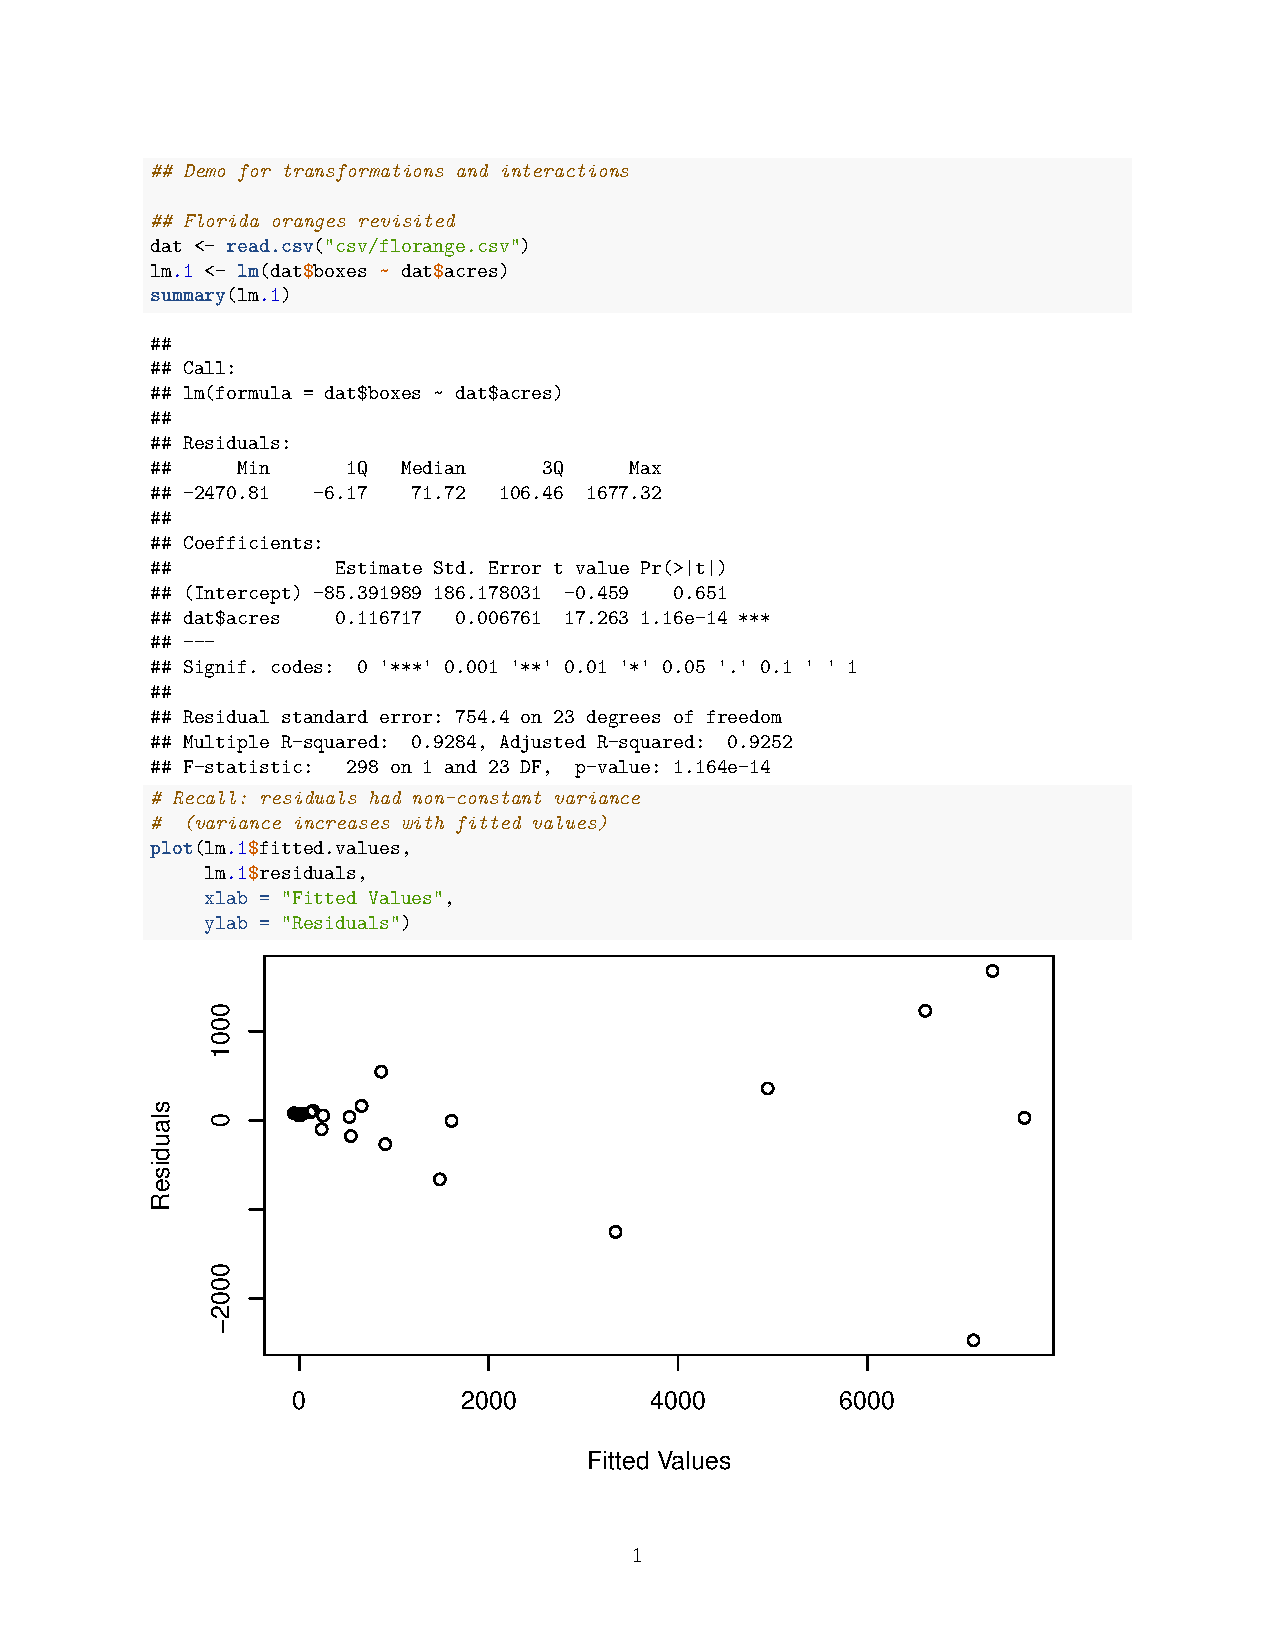
\includepdf[pages=-]{lec_16-demo.pdf}
